\subsection{The Birth of Asymmetric Inference}

The asymmetry of KL divergence was a feature, not a flaw. In fact, it was the breakthrough. It captured something crucial that other metrics --- like Euclidean distance or mean squared error --- couldn’t express. 

\begin{quote}
The cost of being wrong depends on how you’re wrong.
\end{quote}

Suppose you use distribution \( Q \) to approximate the true distribution \( P \). If \( Q \) underestimates rare but important events, you may catastrophically miss them—think of a model that downplays the chance of a system failure or an enemy signal. But if \( Q \) overestimates uncertainty—spreading probability mass too thinly across unlikely outcomes—the consequence might only be inefficiency, not disaster. 

This mismatch is directional. Using \( Q \) to stand in for \( P \) is not the same as using \( P \) to approximate \( Q \). The former corresponds to \textit{modeling reality}; the latter is like asking how surprising the truth would look if your model were right.

That’s what made KL divergence radical: it forced statisticians to choose a direction. To quantify cost, you had to decide which distribution was “truth” and which was “assumption.”

And that’s exactly what Kullback and Leibler did.

\vspace{1em}

\begin{quote}
They weren’t measuring symmetry or balance. They were measuring regret.  The regret you experience when betting on a model \( Q \), only to discover that the world behaves like \( P \). 
\end{quote}

KL divergence gave that regret a unit—\textbf{bits}. Not just metaphorically, but literally: extra bits required to encode truth using the wrong codebook.

In doing so, they laid the groundwork for modern inference, where direction matters. Bayesian updating, variational inference, compression algorithms, even risk-sensitive decision-making—all rely on this asymmetry.

Kullback and Leibler gave the mathematics of expectation a compass. 

\vspace{1em}

\begin{figure}[H]
\centering
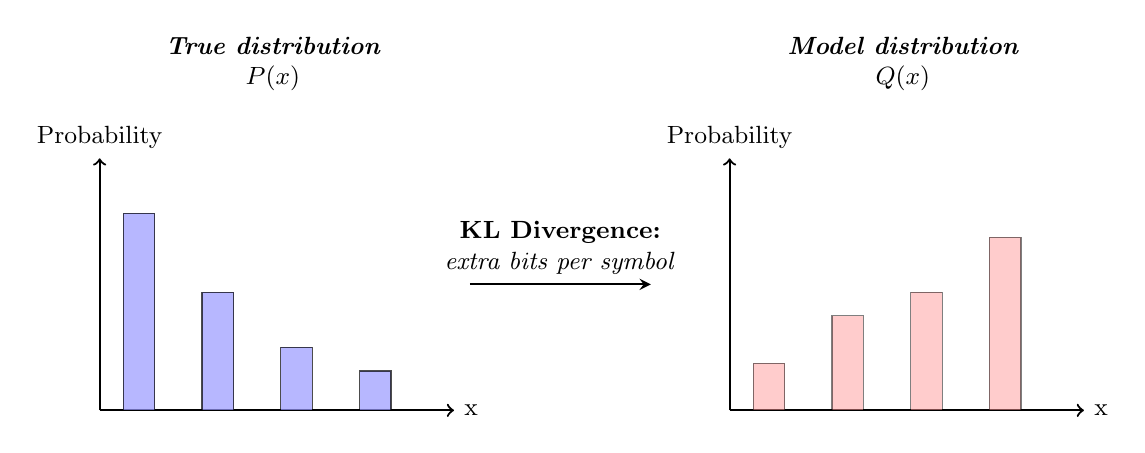
\begin{tikzpicture}[
  every node/.style={font=\small},
  axis/.style={->, thick},
  bar/.style={fill=blue!40, opacity=0.7},
  barq/.style={fill=red!40, opacity=0.5},
  label/.style={font=\small\itshape},
  arrow/.style={->, thick, >=stealth}
]

% Axes for P (left)
\draw[axis] (0,0) -- (4.5,0) node[right] {x};
\draw[axis] (0,0) -- (0,3.2) node[above] {Probability};

% Bars for P
\foreach \x/\h in {0.5/2.5, 1.5/1.5, 2.5/0.8, 3.5/0.5} {
  \draw[bar] (\x-0.2,0) rectangle (\x+0.2,\h);
}

% Label for P
\node[label, align=center] at (2.2,4.4) {\textbf{True distribution} \\ \( P(x) \)};

% Axes for Q (right)
\begin{scope}[xshift=8cm]
\draw[axis] (0,0) -- (4.5,0) node[right] {x};
\draw[axis] (0,0) -- (0,3.2) node[above] {Probability};

% Bars for Q
\foreach \x/\h in {0.5/0.6, 1.5/1.2, 2.5/1.5, 3.5/2.2} {
  \draw[barq] (\x-0.2,0) rectangle (\x+0.2,\h);
}

% Label for Q
\node[label, align=center] at (2.2,4.4) {\textbf{Model distribution} \\ \( Q(x) \)};
\end{scope}

% Arrow indicating KL divergence
\draw[arrow] (4.7,1.6) -- ++(2.3,0) 
  node[midway, above, align=center] {\textbf{KL Divergence:} \\ \textit{extra bits per symbol}};

\end{tikzpicture}
\caption{KL divergence measures the cost of using \( Q \) to approximate \( P \). Even if both are probability distributions over the same space, differences in shape—especially around low-probability but important events—can have real consequences.}
\end{figure}







\begin{figure}[H]
\centering
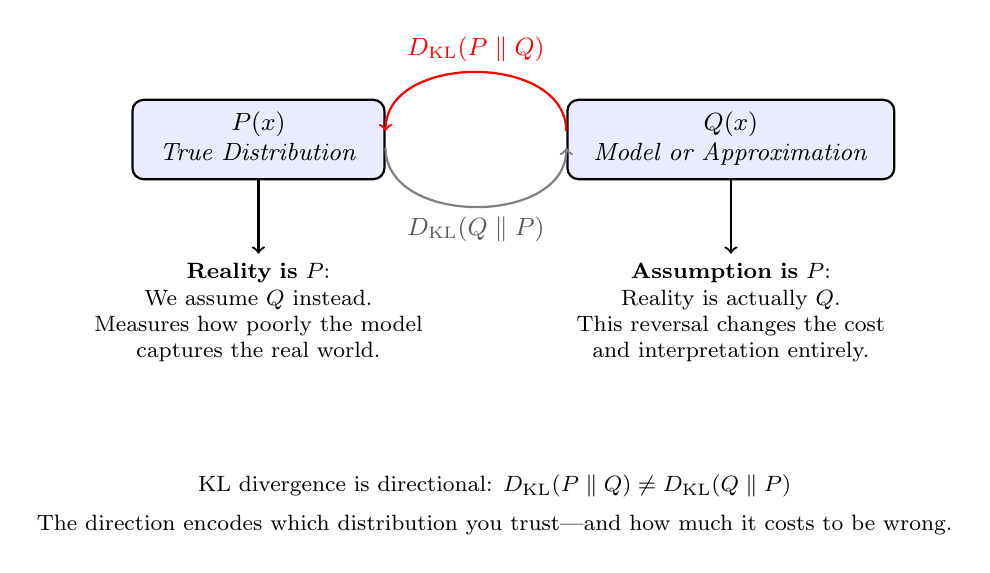
\begin{tikzpicture}[
  every node/.style={font=\small},
  dist/.style={draw, rounded corners, thick, minimum width=3.2cm, minimum height=1cm, fill=blue!8},
  arrow/.style={->, thick},
  explain/.style={align=center, font=\footnotesize, text width=4.2cm}
]

% Explanation boxes first
\node[explain] (e1) at (-3, -2.2) {
  \textbf{Reality is $P$}: \\
  We assume $Q$ instead. \\
  Measures how poorly the model \\
  captures the real world.
};

\node[explain] (e2) at (3, -2.2) {
  \textbf{Assumption is $P$}: \\
  Reality is actually $Q$. \\
  This reversal changes the cost \\
  and interpretation entirely.
};

% Nodes for distributions, vertically above explanations
\node[dist] (P) at (-3,0) {\begin{tabular}{c}$P(x)$\\\textit{True Distribution}\end{tabular}};
\node[dist] (Q) at (3,0) {\begin{tabular}{c}$Q(x)$\\\textit{Model or Approximation}\end{tabular}};

% Curved arrows between P and Q
\draw[->, thick, red]
  ([yshift=3pt] Q.west) .. controls +(up:1cm) and +(up:1cm) .. ([yshift=3pt] P.east)
  node[midway, above, red] {$D_{\mathrm{KL}}(P \parallel Q)$};

\draw[->, thick, gray]
  ([yshift=-3pt] P.east) .. controls +(down:1cm) and +(down:1cm) .. ([yshift=-3pt] Q.west)
  node[midway, below, gray!70!black] {$D_{\mathrm{KL}}(Q \parallel P)$};

% Arrows from dist to explanation
\draw[->, thick] (P.south) -- (e1.north);
\draw[->, thick] (Q.south) -- (e2.north);

% Footer annotation
\node at (0,-4.4) {\footnotesize KL divergence is directional: $D_{\mathrm{KL}}(P \parallel Q) \neq D_{\mathrm{KL}}(Q \parallel P)$};
\node at (0,-4.9) {\footnotesize The direction encodes which distribution you trust—and how much it costs to be wrong.};

\end{tikzpicture}
\caption{KL divergence is asymmetric: assuming the wrong model has different costs depending on the direction.}
\end{figure}







